\section{The cubic alternative}\label{sec:cubic}

We now classify the second alternative of Corollary~\ref{cor:dichotomy}
and complete the proof of Theorem~\ref{thm:fourier}.
Throughout this section, put $\omega=\exp(2\pi i/3)$.
Matrices satisfying the two Hadamard conditions are called S-Hadamard
matrices \cite[Definition~2.1]{Lisonek2019}. The following proposition
proves the order-six classification conjectured by Phangara
\cite[Conjecture~3.1.6]{Phangara2026}. Its representative is the matrix
in Tao's construction \cite[p.~254]{Tao2004}.

\begin{proposition}[Classification of the cubic alternative]
\label{prop:cubic-classification}
Suppose that $H$ and its entrywise square $H^{\circ2}$ are Hadamard
matrices of order six. By multiplying rows and columns by unit complex
numbers and permuting rows and columns, one can transform $H$ into the
matrix $T$ in \eqref{eq:cubic-matrix}.
In particular, every entry of the transformed matrix is a cube root of
unity.
\end{proposition}

\begin{proof}
Let $v=(v_0,\ldots,v_5)$ be the entrywise ratio of two distinct rows of
$H$, and set $p_k(v)=\sum_i v_i^k$. The two Hadamard conditions give
$p_1(v)=p_2(v)=0$. If $e_k$ denotes the $k$th elementary symmetric
function of these six coordinates, Newton's identities give
$e_1=e_2=0$. Since $|v_i|=1$,
\[
 e_{6-k}=e_6\overline{e_k},
\]
so $e_4=e_5=0$ as well. Consequently
\[
 \prod_{i=0}^5(z-v_i)=z^6-e_3z^3+e_6.
\]
Factoring this as a quadratic in $z^3$ shows that the multiset of
coordinates of $v$ is the union of two rotated cube-root triples.
The triples may coincide. Thus the cubed coordinates have either one
value six times or two distinct values three times each. The same
conclusion holds for ratios of columns, because both matrices also
have orthogonal columns.

Dephase $H$, making its initial row and column equal to one. This
preserves both Hadamard conditions. Every row of $H^{\circ3}$ is now
either all ones or has the value $1$ three times and a value $x\ne1$
three times. For a nonconstant row, call the three positions carrying
$x$ its support; its support excludes column zero.

All nonconstant rows have the same support. Indeed, suppose two
distinct supports $S,U$ have respective values $x,y\ne1$, and put
$k=|S\cap U|$. As $S,U$ are three-element subsets of five positions,
$k\in\{1,2\}$. The cubed row ratio has the following values and
multiplicities:
\[
\begin{array}{c|cccc}
\text{value}&1&x&y^{-1}&xy^{-1}\\
\text{multiplicity}&k&3-k&3-k&k.
\end{array}
\]
Every multiplicity is positive, whereas this ratio can have at most two
distinct cubed values. The three values $1,x,y^{-1}$ therefore force
$x=y^{-1}$. Next $xy^{-1}=x^2$ must equal $1$ or $x$, which forces
$x=y=-1$. The two multiplicities would then be $2k$ and $6-2k$, namely
$2$ and $4$ in some order, contradicting the required multiplicities
$3$ and $3$. Applying the same argument to columns proves the
corresponding assertion for their supports.

Suppose that $H^{\circ3}$ is not all ones. Its common nonconstant-row
support consists of three columns. Each of those columns has exactly
three non-one entries, so exactly three rows are nonconstant. Comparing
their values in any one of these columns shows that their non-one
values coincide. After arranging these two classes of rows and columns,
the cubed matrix therefore has the form
\begin{equation}\label{eq:cubic-block}
 H^{\circ3}=\begin{pmatrix}
 J_3&J_3\\ J_3&xJ_3
 \end{pmatrix},\qquad x\ne1,
\end{equation}
where $J_3$ is the all-ones matrix of order three.

Restrict each row of $H$ to the three columns of the $xJ_3$ block.
For rows from opposite classes, the ratio cubes to $x$ or $x^{-1}$ on
these columns and to $1$ on the other three. The two rotated triples
in that ratio are therefore separated by this division of the columns.
Their sums are zero, so the restrictions of rows from opposite classes
are mutually orthogonal.

Each class spans a space of dimension at least two on these three
columns. To see this, suppose that the three restrictions in one class
span a line. Each has squared norm three, so the inner product of any
two has modulus three. Orthogonality of the full rows forces their
complementary restrictions to have inner product of modulus three as
well. Equality in Cauchy--Schwarz makes these complementary restrictions
proportional. The three full rows would then lie in a space of
dimension at most two, contrary to their orthogonality. Thus the two
mutually orthogonal restricted spans have dimensions at least two,
which is impossible in $\C^3$. This excludes
\eqref{eq:cubic-block}. Every entry of the dephased $H$ is consequently
a cube root of unity.

In each noninitial row and column, orthogonality to the initial one
implies that each cube root occurs twice. There is therefore exactly
one additional entry equal to one in each noninitial row and column.
These entries form a matching and may be placed on the diagonal by a
column permutation. Write the other entries as $\omega^{s_{ij}}$, where
$s_{ij}\in\{-1,1\}$ and $i,j\in\{1,\ldots,5\}$ are distinct. Each
such row has two plus signs and two minus signs.

For two distinct noninitial rows $i,j$, their ratio contains each root
twice. They agree at column zero, disagree at columns $i,j$, and hence
agree at exactly one of the remaining three columns. There are thus
two sign mismatches among those three columns, giving
\[
 \prod_{k\notin\{0,i,j\}}s_{ik}s_{jk}=1.
\]
The product of the four signs in each complete noninitial row is also
one. It follows that $s_{ij}s_{ji}=1$, so $s_{ij}=s_{ji}$. The plus
signs define a simple undirected graph of degree two on five vertices.
Its components are cycles of length at least three; therefore it is a
single five-cycle. A simultaneous permutation of the noninitial rows
and columns now gives \eqref{eq:cubic-matrix}; Figure~\ref{fig:cubic-cycle}
shows its two off-diagonal exponent classes.
For completeness, the displayed $T$ is itself Hadamard: every
difference of distinct exponent rows contains each residue modulo
three twice, as seen by separating an initial-row pair, an adjacent
pair on the cycle, and a nonadjacent pair. Its entrywise square is
$\overline T$ and is Hadamard as well.
\end{proof}

\begin{figure}[htbp]
\centering
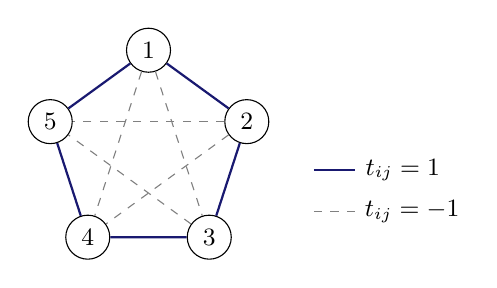
\begin{tikzpicture}[scale=1.05,every node/.style={font=\small}]
  \foreach \i/\angle in {1/90,2/18,3/-54,4/-126,5/162}
    \node[circle,draw,fill=white,inner sep=3pt] (v\i) at (\angle:1.25) {$\i$};
  \foreach \i/\j in {1/3,1/4,2/4,2/5,3/5}
    \draw[dashed,gray] (v\i)--(v\j);
  \foreach \i/\j in {1/2,2/3,3/4,4/5,5/1}
    \draw[thick,MidnightBlue] (v\i)--(v\j);
  \draw[thick,MidnightBlue] (2,-.2)--(2.5,-.2)
    node[right,black] {$t_{ij}=1$};
  \draw[dashed,gray] (2,-.7)--(2.5,-.7)
    node[right,black] {$t_{ij}=-1$};
\end{tikzpicture}
\caption{The five-cycle determining the noninitial off-diagonal entries
of the cubic matrix $T$. Solid edges contribute $\omega$ and dashed edges
contribute $\omega^{-1}$. The diagonal and the initial row and column
consist of ones.}
\label{fig:cubic-cycle}
\end{figure}

The classification also settles the Fourier-vanishing conjecture of
Matolcsi, Ruzsa, and Weiner~\cite[Conjecture~2.3]{MatolcsiRuzsaWeiner2013}.
Here equivalence means multiplication of rows and columns by unit
complex numbers and permutation of rows and columns. The matrix $T$ is
equivalent to the spectral matrix $S_6$ displayed
in~\cite[(93)--(94)]{TadejZyczkowski2006}: with our zero-based indices,
$T_{ij}=(S_6)_{p(i),p(j)}$ for
$(p(0),\ldots,p(5))=(0,1,2,5,4,3)$.

\begin{proof}[Proof of Theorem~\ref{thm:fourier}]
If $g_H(\pi\alpha)$ were nonzero for some coordinate permutation $\pi$,
Corollary~\ref{cor:dichotomy} would imply that $H^{\circ2}$ is
Hadamard. Proposition~\ref{prop:cubic-classification} would then make
$H$ equivalent to $T$, a contradiction.
\end{proof}

